\chapter{Программная реализация}

При разработке широко использовалось модульное программирования. При чём в некоторых частях программы использовались
продвинутые возможности языка модулей ML (реализованный в используемом OCaml), которые позволяют
отделять интерфейс модуля от его реализации,
параметризировать модули другими модулями (образуя функторы),
включать один модуль в другой, \cite{wiki-mlmodules}
производить инъекцию зависимостей и т.д \cite{functor-driven}.

Например, функторы были использованы для того чтобы в реализации численного метода решения алгебраических уравнений
от конкретной реализации вещественных чисел. Это позволяет абстрагироваться от конкретной реализации вещественных,
что позволит на деле использовать разные реализации, например модуль для работы с числами двойной точности из стандартной библиотеки,
или самописную реализацию с использованием дробей на основе чисел двойной точности, или реализацию на основе длинной арифметики.

Была попытка использовать функторы и при реализации движка, но при чрезмерном их использовании код усложняется и для разработчика,
и для компилятора: слишком долгая компиляция, анализатор кода для интегрированной среды разработки потребляет слишком много памяти.
Поэтому сам движок разработан баз использования функторов: для представления вещественных чисел используются числа
с плавающей запятой двойной точности (в OCaml он называется <<float>>, когда в других языках может быть известен как <<double>>).

Проект состоит из нескольких подпроектов. На рисунке~\ref{libsdiagramfig} представлена диаграмма зависимостей между ними.
В таблице~\ref{libstable} указано их место в исходном коде и соответствующий пункт ВКР.

\pagebreak
\begin{figure}[H]
    \centering
    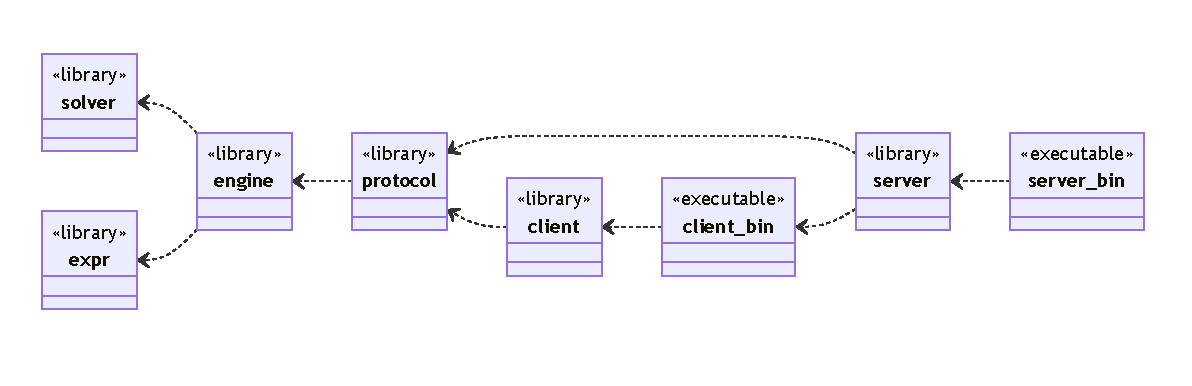
\includegraphics[width=15cm]{libsdiagram}
    \caption{Диаграмма зависимостей подпроектов\label{libsdiagramfig}}
\end{figure}

\begin{centering}
    \begin{longtable}{|l|l|l|}
        \caption{Подпроекты} \label{libstable}                                                                                                                                                 \\

        \hline \multicolumn{1}{|c|}{\textbf{Название подпроекта}} & \multicolumn{1}{c|}{\textbf{Каталог}}                                            & \multicolumn{1}{c|}{\textbf{Пункт ВКР}} \\ \hline
        \endfirsthead

        \multicolumn{3}{c}%
        {\hspace{-12.5cm}{Окончание таблицы \thetable} \vspace{1ex}}                                                                                                                           \\
        \hline \multicolumn{1}{|c|}{\textbf{Название подпроекта}} & \multicolumn{1}{c|}{\textbf{Каталог}}                                            & \multicolumn{1}{c|}{\textbf{Пункт ВКР}} \\ \hline
        \endhead

        solver                                                    & \href{https://github.com/prekel/chapgame/blob/master/lib/solver}{lib/solver}     & \ref{solverimpl}                        \\ \hline
        expr                                                      & \href{https://github.com/prekel/chapgame/blob/master/lib/expr}{lib/expr}         & \ref{expr}                              \\ \hline
        engine                                                    & \href{https://github.com/prekel/chapgame/blob/master/lib/engine}{lib/engine}     & \ref{engine}                            \\ \hline
        protocol                                                  & \href{https://github.com/prekel/chapgame/blob/master/lib/protocol}{lib/protocol} & \ref{clientonlineimpl}                  \\ \hline
        server                                                    & \href{https://github.com/prekel/chapgame/blob/master/lib/server}{lib/server}     & \multirow{2}{*}{\ref{serverimpl}}       \\*
        server\_bin                                               & \href{https://github.com/prekel/chapgame/blob/master/bin/server}{bin/server}     &                                         \\ \hline
        client                                                    & \href{https://github.com/prekel/chapgame/blob/master/lib/client}{lib/client}     & \multirow{2}{*}{\ref{clientimpl}}       \\*
        client\_bin                                               & \href{https://github.com/prekel/chapgame/blob/master/bin/client}{bin/client}     &                                         \\ \hline
    \end{longtable}
\end{centering}

На рисунках~\ref{solvermodules} и~\ref{exprdiagramfig} представлены диаграммы с функторами,
ромбовидная стрелка из \(F\) в \(S\) означает, что функтор \(F\) параметризируется модулем, имеющим сигнатуру \(S\);
треугольная стрелка из \(F\) в \(S\) означает, что функтор \(F\) возвращает модуль с сигнатурой \(S\).
Так как функторы можно назвать параметризированными модулями, далее функторы будут называться модулями.

\section{Реализация метода решения алгебраических уравнений}\label{solverimpl}

Диаграмма модулей приведена на рисунке~\ref{solvermodules}. В таблице~\ref{solvermodulestable} показано их место в реализации и расшифровка.

\begin{figure}[H]
    \centering
    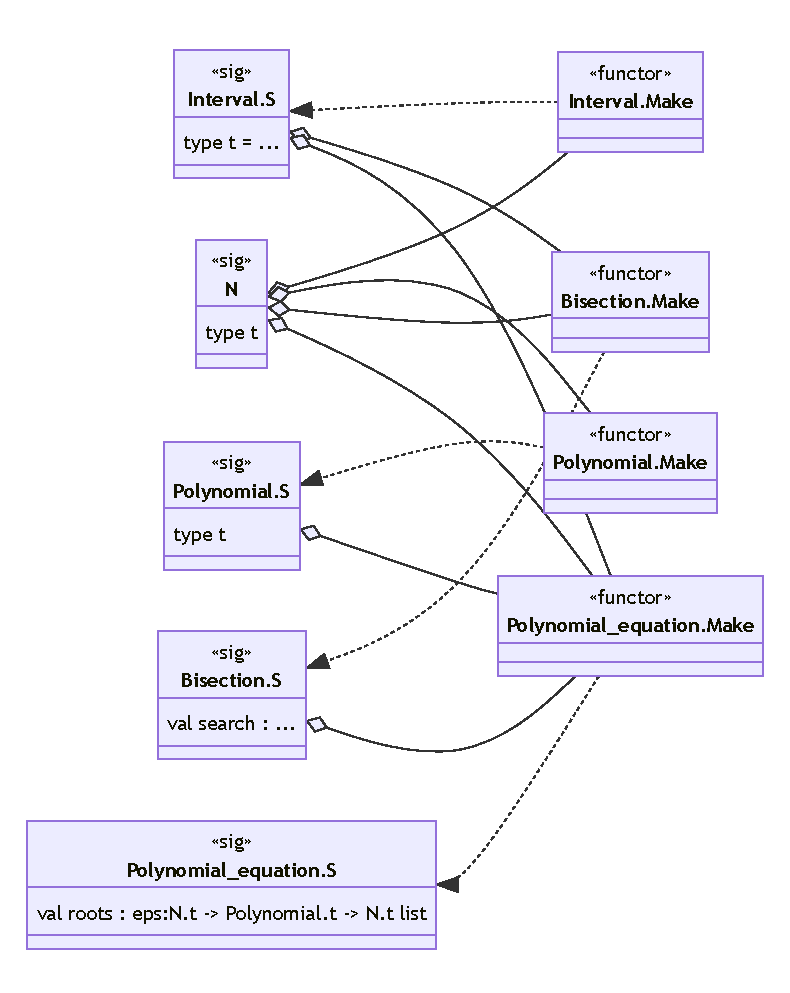
\includegraphics[width=10cm]{solver}
    \caption{Диаграмма модулей решателя алгебраических уравнений\label{solvermodules}}
\end{figure}

\begin{centering}
    \begin{longtable}{|l|l|l|}
        \caption{Модули решателя алгебраических уравнений} \label{solvermodulestable}                                                                                                                                                                    \\

        \hline \multicolumn{1}{|c|}{\textbf{Название модуля}} & \multicolumn{1}{c|}{\textbf{Файлы}}                                                                                                      & \multicolumn{1}{c|}{\textbf{Расшифровка}}     \\ \hline
        \endfirsthead

        \multicolumn{3}{c}%
        {\hspace{-12.5cm}{Окончание таблицы \thetable} \vspace{1ex}}                                                                                                                                                                                     \\
        \hline \multicolumn{1}{|c|}{\textbf{Название модуля}} & \multicolumn{1}{c|}{\textbf{Файлы}}                                                                                                      & \multicolumn{1}{c|}{\textbf{Расшифровка}}     \\ \hline
        \endhead

        \multirow{2}{*}{Interval}                             & \href{https://github.com/prekel/chapgame/blob/master/lib/solver/interval.ml}{lib/solver/interval.ml}                                     & \multirow{2}{*}{Промежуток}                   \\*
                                                              & \href{https://github.com/prekel/chapgame/blob/master/lib/solver/interval\_intf.ml}{lib/solver/interval\_intf.ml}                         &                                               \\ \hline
        \multirow{2}{*}{Polynomial}                           & \href{https://github.com/prekel/chapgame/blob/master/lib/solver/polynomial.ml}{lib/solver/polynomial.ml}                                 & \multirow{2}{*}{Многочлен}                    \\*
                                                              & \href{https://github.com/prekel/chapgame/blob/master/lib/solver/polynomial\_intf.ml}{lib/solver/polynomial\_intf.ml}                     &                                               \\ \hline
        \multirow{2}{*}{Bisection}                            & \href{https://github.com/prekel/chapgame/blob/master/lib/solver/bisection.ml}{lib/solver/bisection.ml}                                   & \multirow{2}{*}{Бисекция}                     \\*
                                                              & \href{https://github.com/prekel/chapgame/blob/master/lib/solver/bisection\_intf.ml}{lib/solver/bisection\_intf.ml}                       &                                               \\ \hline
        \multirow{2}{*}{Polynomial\_equation}                 & \href{https://github.com/prekel/chapgame/blob/master/lib/solver/polynomial\_equation.ml}{lib/solver/polynomial\_equation.ml}             & \multirow{2}{3.4cm}{Алгебраическое уравнение} \\*
                                                              & \href{https://github.com/prekel/chapgame/blob/master/lib/solver/polynomial\_equation\_intf.ml}{lib/solver/polynomial\_equation\_intf.ml} &                                               \\ \hline
    \end{longtable}
\end{centering}

\textbf{Промежуток}. Промежуток представлен алгебраическим типом данных
(алгебраический тип данных в функциональном программировании~-- размеченное объединение
других типов \cite{fprog-adt}),
у которого есть несколько конструкторов:

\begin{itemize}
    \item от одного вещественного числа до другого;
    \item от \(-\infty\) до заданного вещественного числа;
    \item от заданного вещественного числа до \(+\infty\);
    \item от \(-\infty\) до \(+\infty\) (вся числовая прямая);
    \item пустой промежуток.
\end{itemize}

Так же в этом модуле представлены функции для конвертации в кортеж, создания промежутка,
разбиения списка значений на промежутки, вычисления разности между правым и левым значением.

\textbf{Многочлен}. Многочлен представлен иммутабельным словарём, ключом которого является целое число (представляющее степень одночлена),
значением является вещественное число (представляющее коэффициент одночлена).
Предоставляет функции для создания многочлена из списка кортежей, для вычисления производной многочлена, для вычисления степени многочлена.
На рисунке~\ref{derivativecode} представлена для примера реализация функции вычисления производной многочлена. Её можно прочитать так:
<<Пары ключ-значения из словаря, которым представлен многочлен, фильтруются так, чтобы остались только с ненулевой степенью,
и заодно коэффициент преобразовывается в коэффициент производной, умножаясь на степень; далее все ключи отображаются так, чтобы стали на единицу меньше
(при этом степень не может стать отрицательной, потому что многочлен нельзя создать с отрицательной степенью у одночлена,
а на предыдущем шаге мы исключили одночлен с нулевой степенью)>>.

\begin{figure}[H]
    \centering
    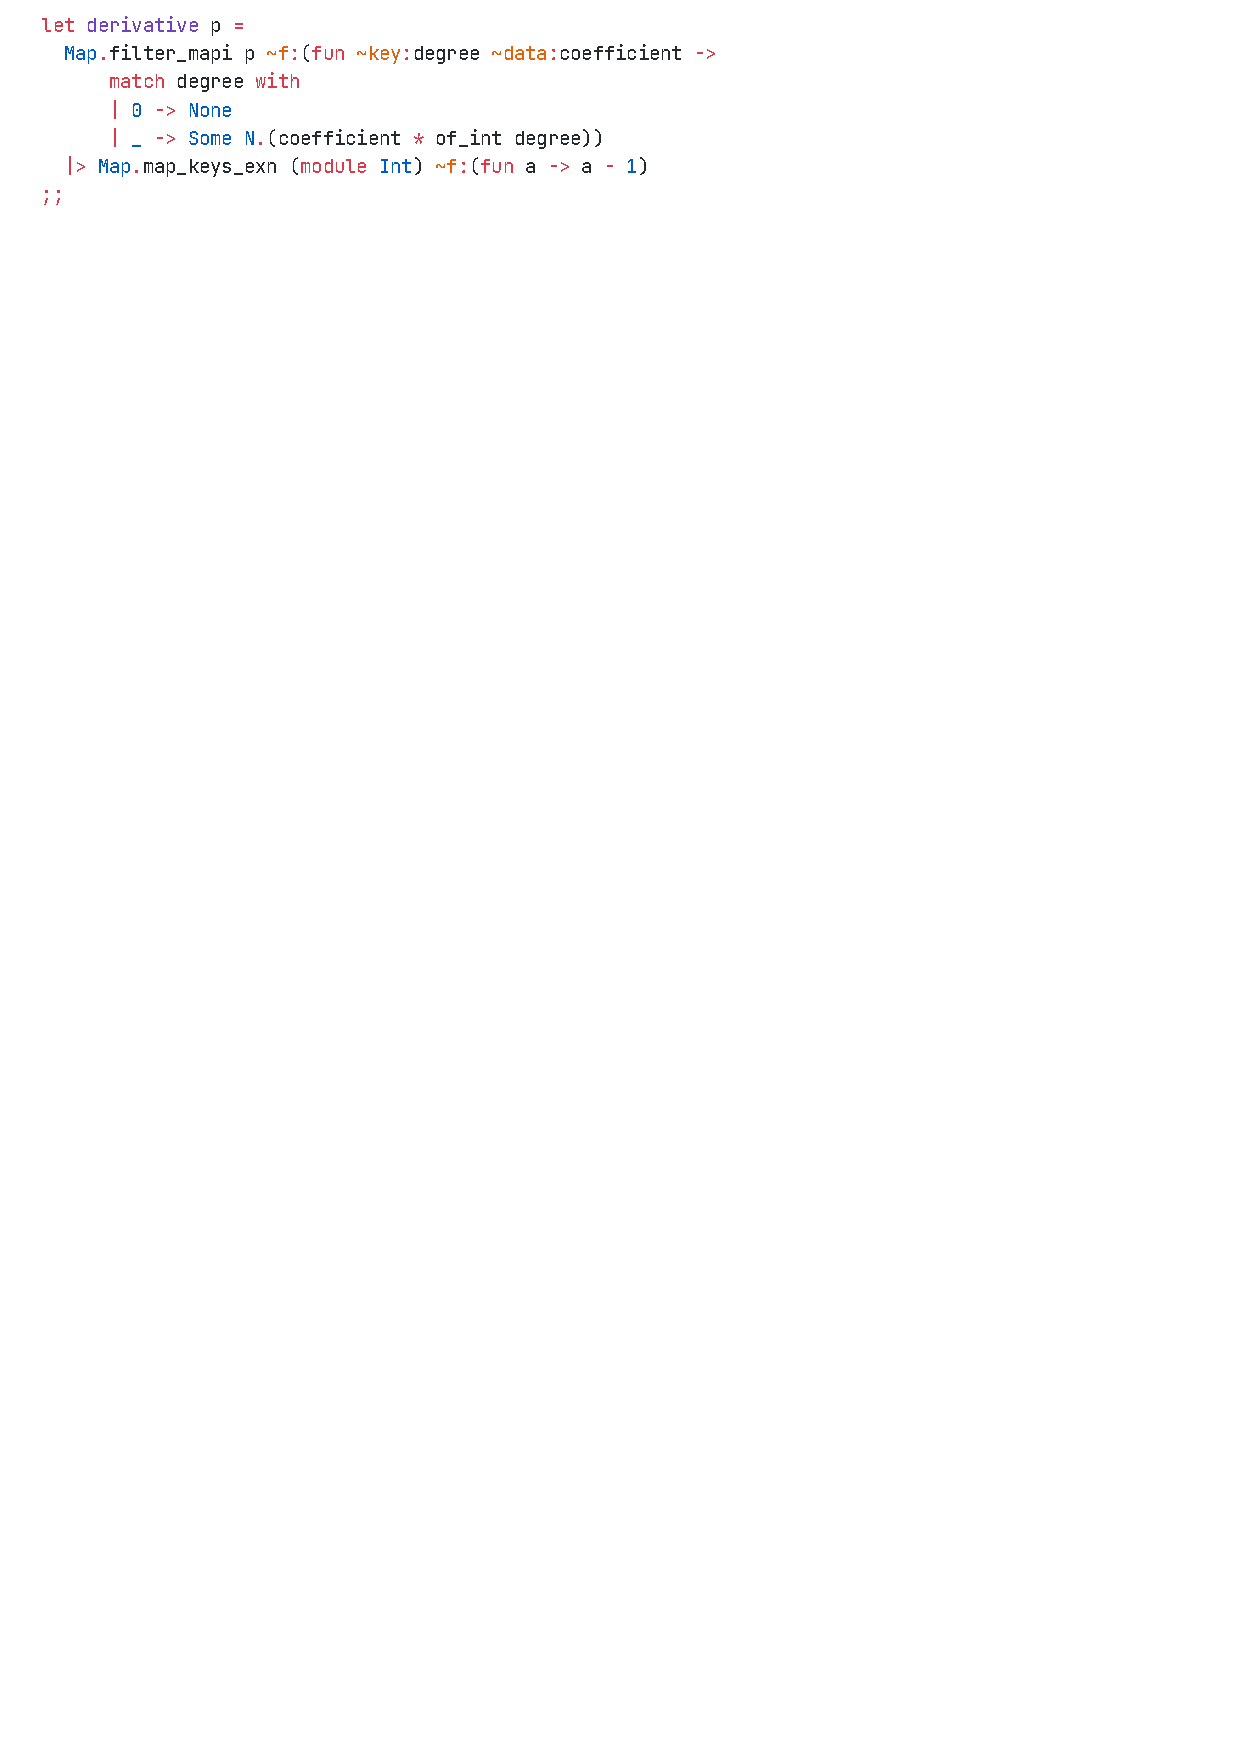
\includegraphics[width=12cm]{derivative}
    \caption{Реализация функции нахождения производной многочлена\label{derivativecode}}
\end{figure}

\textbf{Бисекция}. Этот модуль представляет функцию, принимающую другую функцию \(f(x)\), точность \(\varepsilon\)
и промежуток, на котором надо искать такой \(x\), что \(\left|f(x)\right| < \varepsilon\). Предполагается, что
функция монотонно возрастает или убывает на требуемом промежутке. Кроме самого метода бисекции, в ней реализован алгоритм,
позволяющий находить значения на бесконечном и полубесконечном промежутке, который описан в пункте~\ref{bisection}.

\textbf{Алгебраическое уравнение}. Этот модуль, используя все 3 вышеописанных, предоставляет главную функцию~-- принимающую
точность вычислений \(\varepsilon\) и многочлен \(P(x)\), и возвращающую список таких \(x\), что \(\left|P(x)\right| < \varepsilon\).
Иными словами, решает алгебраическое уравнение заданное многочленом с заданной точностью. На рисунке~\ref{rootscode}
представлена её реализация, её можно прочитать следующим образом:
<<Вычисляется степень многочлена.
Если она нулевая или отрицательная, то вернуть пустой список.
Если равна единице, решить как линейное уравнение и преобразовать в список.
Если равна двум, решить как квадратное уравнение, учитывая точность.
Иначе, вычислить производную многочлена и найти её корни; разбить список корней на промежутки и методом бисекции найти корни на промежутках>>.

\begin{figure}[H]
    \centering
    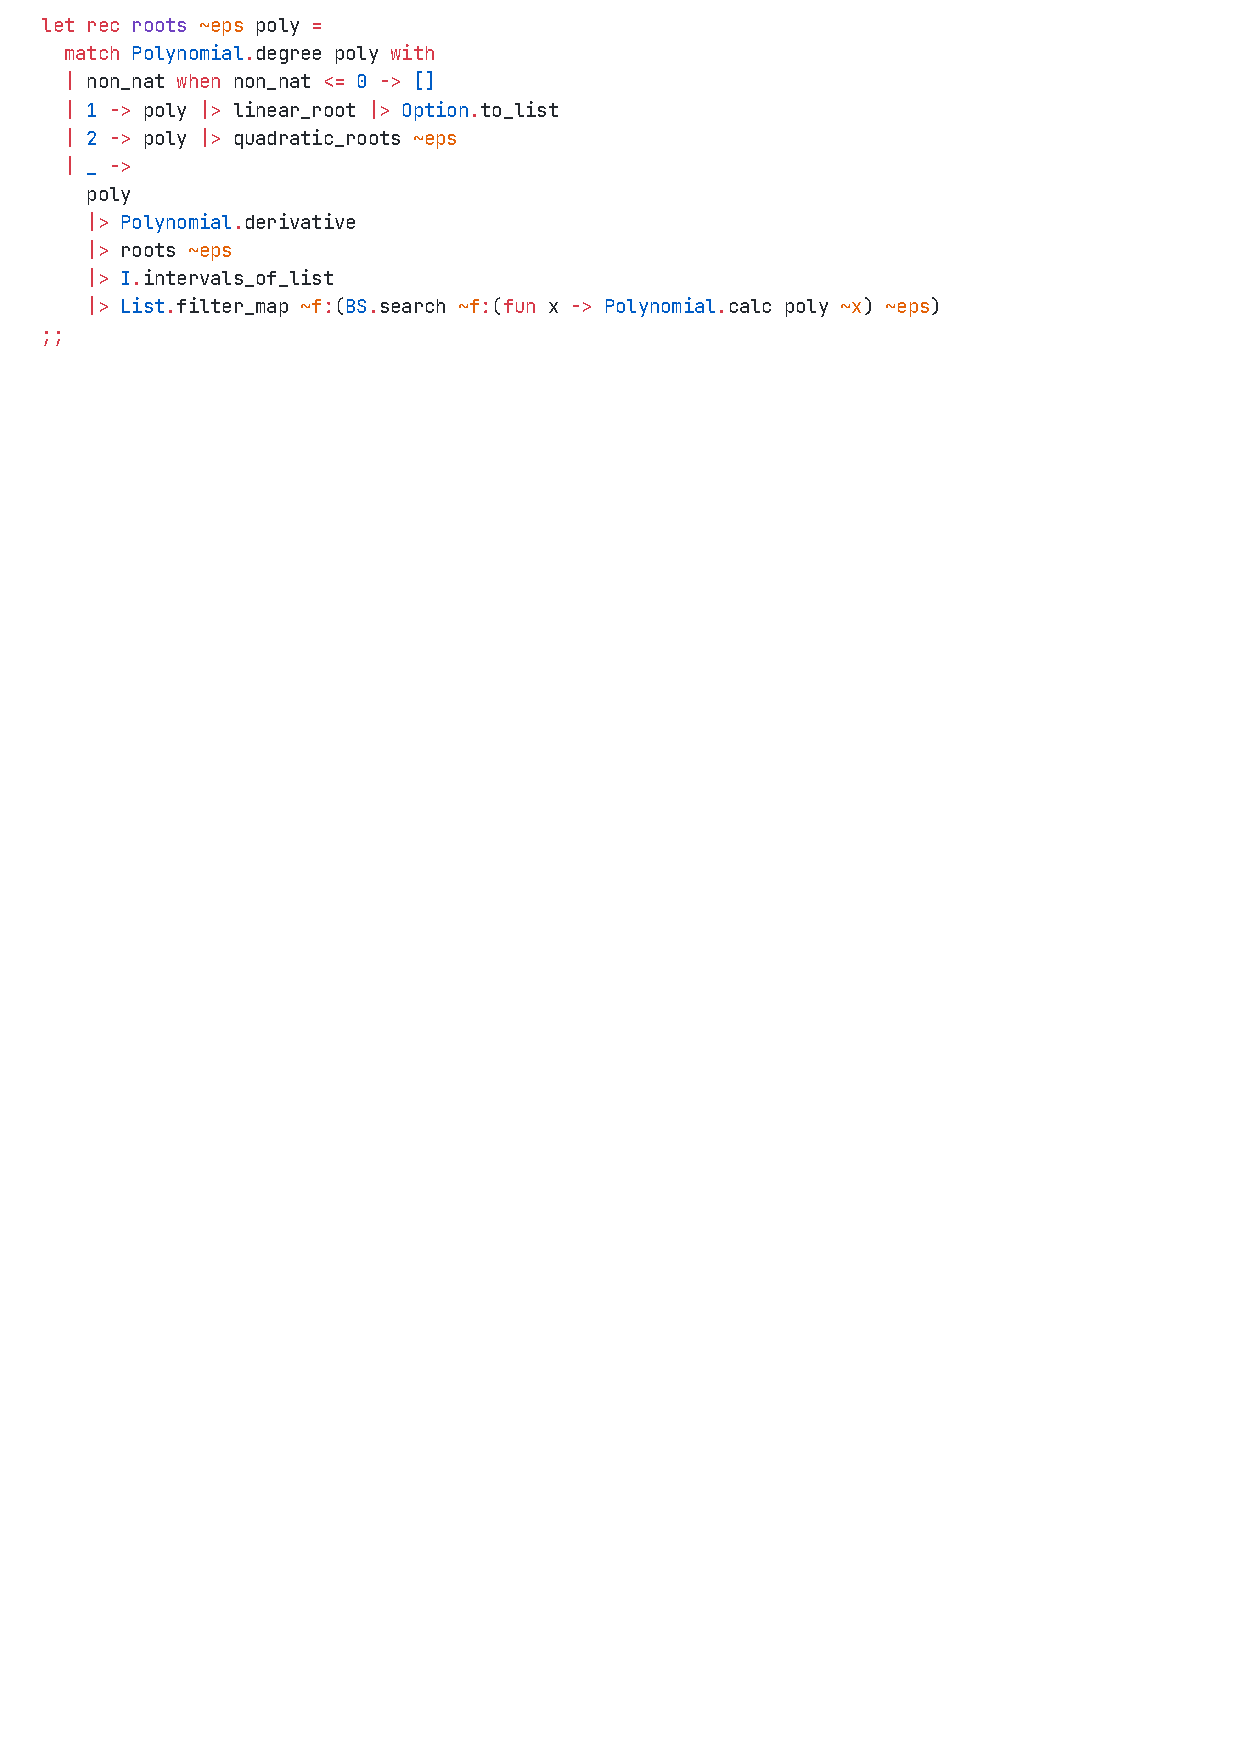
\includegraphics[width=14cm]{roots}
    \caption{Реализация функции нахождения корней алгебраического уравнения\label{rootscode}}
\end{figure}

Таким образом, реализован метод численного решения алгебраических уравнений, описанный в пункте~\ref{solvefourthdegree}.

\section{Символьные вычисления}\label{expr}

Это часть проекта призвана обобщить вычисление коэффициентов одночленов, когда требуется перемножать или складывать многочлены.
Выражения можно строить из других выражений, вычислять значения подставляя значения на место переменных в подвыражениях.
Выражения-многочлены можно складывать и перемножать, а так же вычисляя значения коэффициентов, приводить в вид многочлена,
на основе которого решается алгебраическое уравнение.
Диаграмма модулей приведена на рисунке~\ref{exprdiagramfig}. В таблице~\ref{exprtable} показано их место в реализации и расшифровка.

\begin{figure}[H]
    \centering
    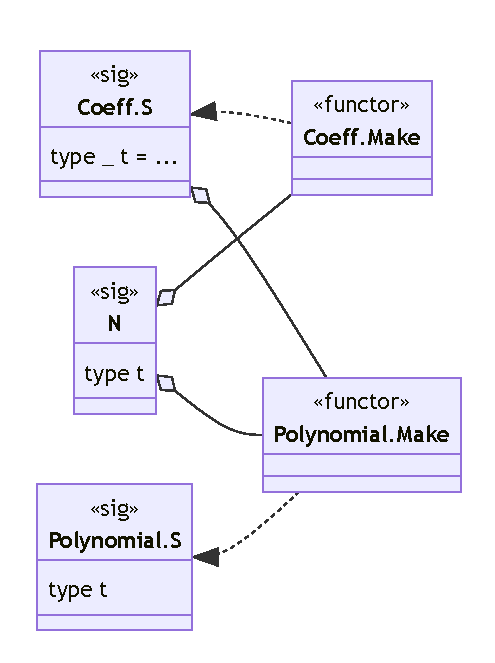
\includegraphics[width=8cm]{exprdiagram}
    \caption{Диаграмма модулей библиотеки символьных вычислений\label{exprdiagramfig}}
\end{figure}

\begin{centering}
    \begin{longtable}{|l|l|l|}
        \caption{Модули библиотеки символьных вычислений} \label{exprtable}                                                                                                                                                  \\

        \hline \multicolumn{1}{|c|}{\textbf{Название модуля}} & \multicolumn{1}{c|}{\textbf{Файлы}}                                                                              & \multicolumn{1}{c|}{\textbf{Расшифровка}} \\ \hline
        \endfirsthead

        \multicolumn{3}{c}%
        {\hspace{-12.5cm}{Окончание таблицы \thetable} \vspace{1ex}}                                                                                                                                                         \\
        \hline \multicolumn{1}{|c|}{\textbf{Название модуля}} & \multicolumn{1}{c|}{\textbf{Файлы}}                                                                              & \multicolumn{1}{c|}{\textbf{Расшифровка}} \\ \hline
        \endhead

        \multirow{2}{*}{Coeff}                                & \href{https://github.com/prekel/chapgame/blob/master/lib/expr/coeff.ml}{lib/expr/coeff.ml}                       & \multirow{2}{*}{Выражение}                \\*
                                                              & \href{https://github.com/prekel/chapgame/blob/master/lib/expr/coeff\_intf.ml}{lib/expr/coeff\_intf.ml}           &                                           \\ \hline
        \multirow{2}{*}{Polynomial}                           & \href{https://github.com/prekel/chapgame/blob/master/lib/expr/polynomial.ml}{lib/expr/polynomial.ml}             & \multirow{2}{*}{Выражение-многочлен}      \\*
                                                              & \href{https://github.com/prekel/chapgame/blob/master/lib/expr/polynomial\_intf.ml}{lib/expr/polynomial\_intf.ml} &                                           \\ \hline
    \end{longtable}
\end{centering}

\textbf{Выражение}. Представлено обобщённым алгебраическим типом данным (GADT), так как для вычисления уравнений требуется
оперировать и скалярными, и векторными величинами. GADT позволяют построить тип так, чтобы статически разграничить выражения,
результатом вычисления которых являются скалярные или векторные величины~\cite{rwo-gadt}. При этом, для построения выражений, скалярные выражения
могут использовать векторные, и наоборот, в зависимости от операции. Например, операция, получающая проекцию вектора на ось \(X\) (<<XOfVector>>),
принимает векторное выражение и возвращает скалярное; а операция для получения вектора из его проекций, получает обе его проекции в виде скалярных выражений
и возвращает векторное выражение (рисунок~\ref{exprgadtcode}). Такая структура является деревом, а его листья это либо константы, либо
переменные, идентифицируемые отдельным типом. При этом если и полиморфные операции, такие как сумма или унарный минус, возвращающие выражение
такого же типа, что и принимают. Кроме того, есть операция <<Scope>>, позволяющая как-бы <<навесить>> нижний индекс на все переменные,
и при вычислении значения переменной, потребуется так же указать этот индекс, помимо имени переменной и её значения.

\begin{figure}[H]
    \centering
    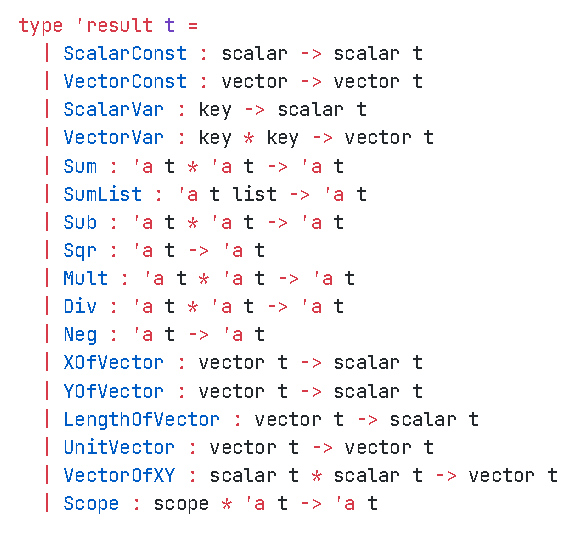
\includegraphics[width=10cm]{exprgadt}
    \caption{Определение типа выражения\label{exprgadtcode}}
\end{figure}

Чтобы не строить выражения напрямую из конструкторов, были определены отдельные функции, в том числе инфиксные операторы для операций сложения, вычитания и т.д.,
что позволило записывать выражения в привычном виде. На рисунке~\ref{exprtestfig} представлен юнит-тест, в котором строится выражение~(\ref{samleexpr}) и вычисляется
его значение при \(x = 24\) и \(y = 4\).

\begin{equation}\label{samleexpr}
    \frac{xy - x + 8}{y^2}
\end{equation}

\vspace{-2em}

\begin{figure}[H]
    \centering
    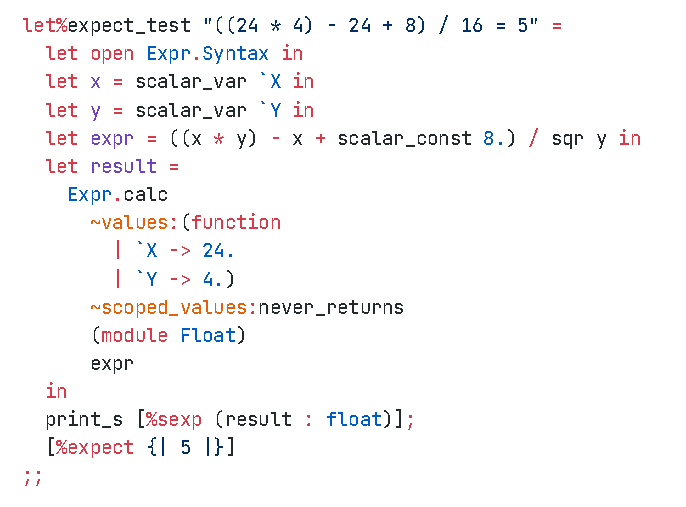
\includegraphics[width=10cm]{exprtest}
    \caption{Реализация юнит-теста для выражения\label{exprtestfig}}
\end{figure}

\textbf{Выражение-многочлен}. Этот модуль представляет одноместный многочлен, коэффициентами которого
являются выражения, описанные ранее. Для представления используется иммутабельный словарь, ключами которого являются целые числа~-- степень одночлена,
значения~-- выражения, описывающие коэффициенты этого одночлена. Пример использования: на рисунке~\ref{exprpolytestcode} представлен юнит-тест, в котором строится
многочлен~(\ref{samplepolyexpr}) и подставляются \(x = 24\) и \(y = 4\).

\begin{align}\label{samplepolyexpr}
    P_1(t) & = (-x + y)t^2 + (x \cdot (-y))t \nonumber           \\
    P_2(t) & = (x - y)t^2 + (x \cdot (-y))t + (-x + y) \nonumber \\
    P_1(t) & P_2(t) - P_1(t) + P_2(t)
\end{align}

\begin{figure}[H]
    \centering
    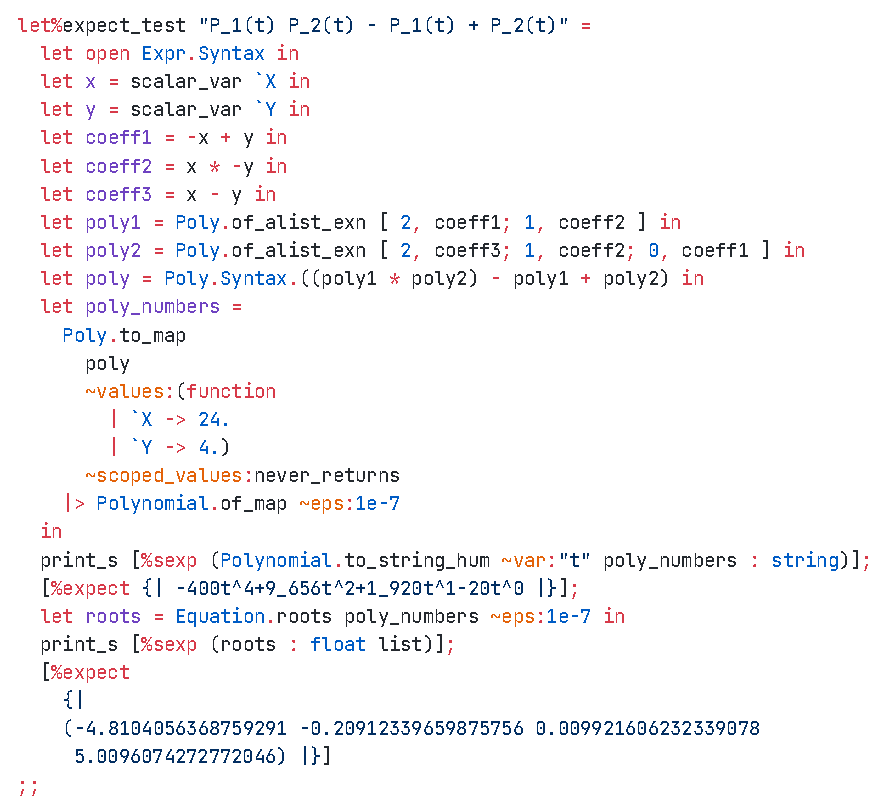
\includegraphics[width=10cm]{exprpolytest}
    \caption{Реализация юнит-теста в котором строится многочлен~(\ref{samplepolyexpr})\label{exprpolytestcode}}
\end{figure}

Из рисунка~\ref{exprpolytestcode} видно, что получен многочлен~(\ref{resultsamplepoly}) и его корни это \(x~\approx~-4.8104, x~\approx~-0.2091, x~\approx~0.0099, x~\approx~5.0096\). 

\begin{equation}\label{resultsamplepoly}
    -400t^4 + 9656t^2 + 1920t - 20
\end{equation}

На рисунке~\ref{samplepolyplotfig} представлен график соответствующего уравнения, где видно примерное расположение корней.

\begin{figure}[H]
    \centering
    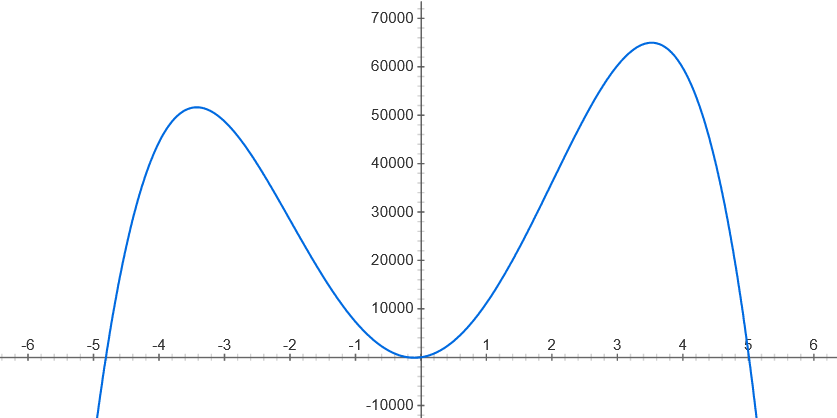
\includegraphics[width=13cm]{samplepolyplot}
    \caption{График многочлена~(\ref{resultsamplepoly})\label{samplepolyplotfig}}
\end{figure}

\section{Движок}\label{engine}

Архитектура движка имеет более плоскую и последовательную структуру, поэтому нет смысла приводить диаграмму.
В таблице~\ref{enginemodules} представлены названия модулей и файлы модулей, далее описана их работа.

\begin{centering}
    \begin{longtable}{|l|l|l|}
        \caption{Модули движка} \label{enginemodules}                                                                                                                                                                                        \\

        \hline \multicolumn{1}{|c|}{\textbf{Название модуля}} & \multicolumn{1}{c|}{\textbf{Файлы}}                                                                                            & \multicolumn{1}{c|}{\textbf{Расшифровка}}   \\ \hline
        \endfirsthead

        \multicolumn{3}{c}%
        {\hspace{-12.5cm}{Окончание таблицы \thetable} \vspace{1ex}}                                                                                                                                                                         \\
        \hline \multicolumn{1}{|c|}{\textbf{Название модуля}} & \multicolumn{1}{c|}{\textbf{Файлы}}                                                                                            & \multicolumn{1}{c|}{\textbf{Расшифровка}}   \\ \hline
        \endhead

        \hline
        \endfoot

        \multirow{2}{*}{Point}                                & \href{https://github.com/prekel/chapgame/blob/master/lib/engine/point.ml}{lib/engine/point.ml}                                 & \multirow{2}{*}{Точка}                      \\*
                                                              & \href{https://github.com/prekel/chapgame/blob/master/lib/engine/point.mli}{lib/engine/point.mli}                               &                                             \\ \hline
        \multirow{2}{*}{Line}                                 & \href{https://github.com/prekel/chapgame/blob/master/lib/engine/line.ml}{lib/engine/line.ml}                                   & \multirow{2}{*}{Линия}                      \\*
                                                              & \href{https://github.com/prekel/chapgame/blob/master/lib/engine/line.mli}{lib/engine/line.mli}                                 &                                             \\ \hline
        \multirow{2}{*}{Values}                               & \href{https://github.com/prekel/chapgame/blob/master/lib/engine/values.ml}{lib/engine/values.ml}                               & \multirow{2}{*}{Значения}                   \\*
                                                              & \href{https://github.com/prekel/chapgame/blob/master/lib/engine/values.mli}{lib/engine/values.mli}                             &                                             \\ \hline
        \multirow{2}{*}{Rule}                                 & \href{https://github.com/prekel/chapgame/blob/master/lib/engine/rule.ml}{lib/engine/rule.ml}                                   & \multirow{2}{*}{Правило}                    \\*
                                                              & \href{https://github.com/prekel/chapgame/blob/master/lib/engine/rule.mli}{lib/engine/rule.mli}\TODO                            &                                             \\ \hline
        \multirow{2}{*}{Body}                                 & \href{https://github.com/prekel/chapgame/blob/master/lib/engine/body.ml}{lib/engine/body.ml}                                   & \multirow{2}{*}{Тело}                       \\*
                                                              & \href{https://github.com/prekel/chapgame/blob/master/lib/engine/body.mli}{lib/engine/body.mli}                                 &                                             \\ \hline
        \multirow{2}{*}{Bodies}                               & \href{https://github.com/prekel/chapgame/blob/master/lib/engine/bodies.ml}{lib/engine/bodies.ml}                               & \multirow{2}{*}{Тела}                       \\*
                                                              & \href{https://github.com/prekel/chapgame/blob/master/lib/engine/bodies.mli}{lib/engine/bodies.mli}                             &                                             \\ \hline
        \multirow{2}{*}{Collision\_detection}                 & \href{https://github.com/prekel/chapgame/blob/master/lib/engine/collision\_detection.ml}{lib/engine/collision\_detection.ml}   & \multirow{2}{2cm}{Обнаружение столкновений} \\*
                                                              & \href{https://github.com/prekel/chapgame/blob/master/lib/engine/collision\_detection.mli}{lib/engine/collision\_detection.mli} &                                             \\ \hline
        \multirow{2}{*}{Collision\_handle}                    & \href{https://github.com/prekel/chapgame/blob/master/lib/engine/collision\_handle.ml}{lib/engine/collision\_handle.ml}         & \multirow{2}{*}{Обработка ударов}           \\*
                                                              & \href{https://github.com/prekel/chapgame/blob/master/lib/engine/collision\_handle.mli}{lib/engine/collision\_handle.mli}       &                                             \\ \hline
        \multirow{2}{*}{Scene}                                & \href{https://github.com/prekel/chapgame/blob/master/lib/engine/scene.ml}{lib/engine/scene.ml}                                 & \multirow{2}{*}{Сцена}                      \\*
                                                              & \href{https://github.com/prekel/chapgame/blob/master/lib/engine/scene.mli}{lib/engine/scene.mli}\TODO                          &                                             \\ \hline
        \multirow{2}{*}{Scenes}                               & \href{https://github.com/prekel/chapgame/blob/master/lib/engine/scenes.ml}{lib/engine/scenes.ml}                               & \multirow{2}{*}{Сцены}                      \\*
                                                              & \href{https://github.com/prekel/chapgame/blob/master/lib/engine/scenes.mli}{lib/engine/scenes.mli}                             &                                             \\ \hline
        \multirow{2}{*}{Action}                               & \href{https://github.com/prekel/chapgame/blob/master/lib/engine/action.ml}{lib/engine/action.ml}                               & \multirow{2}{*}{Действие}                   \\*
                                                              & \href{https://github.com/prekel/chapgame/blob/master/lib/engine/action.mli}{lib/engine/action.mli}                             &                                             \\ \hline
        \multirow{2}{*}{Model}                                & \href{https://github.com/prekel/chapgame/blob/master/lib/engine/model.ml}{lib/engine/model.ml}                                 & \multirow{2}{*}{Модель}                     \\*
                                                              & \href{https://github.com/prekel/chapgame/blob/master/lib/engine/model.mli}{lib/engine/model.mli}                               &                                             \\ \hline
        \multirow{2}{*}{Engine}                               & \href{https://github.com/prekel/chapgame/blob/master/lib/engine/engine.ml}{lib/engine/engine.ml}                               & \multirow{2}{*}{Движок}                     \\*
                                                              & \href{https://github.com/prekel/chapgame/blob/master/lib/engine/engine.mli}{lib/engine/engine.mli}                             &                                             \\ \hline
    \end{longtable}
\end{centering}

\textbf{Точка}. \TODO

\textbf{Линия}. \TODO

\textbf{Значения}. \TODO

\textbf{Правило}. \TODO

\textbf{Тело} и \textbf{тела}. \TODO

\textbf{Обнаружение столкновений}. \TODO

\textbf{Обработка ударов}. \TODO

\textbf{Сцена} и \textbf{сцены}. \TODO

\textbf{Действие}. \TODO

\textbf{Модель}. \TODO

\textbf{Движок}. \TODO

\TODO

\section{Клиентская часть, одиночный режим}\label{clientimpl}

\TODO

\section{Серверная часть}\label{serverimpl}

\subsection{Получение отличий модели}\label{model-diff-implementation}

\TODO

\section{Клиентская часть, многопользовательский режим}\label{clientonlineimpl}

\TODO
